\documentclass[conference]{IEEEtran}
\usepackage{cite}
\usepackage{graphicx}
\usepackage{placeins}
\usepackage{float}
\usepackage{subfigure}
\begin{document}
\title{Projeto 1 de Introdu\c{c}\~ao ao Processamento de Imagens \\ Primeira Parte}
\author{\IEEEauthorblockN{Gabriel Martins de Miranda}
\IEEEauthorblockA{130111350\\
Universidade de Bras\'ilia\\
Email:gabrielmirandat@hotmail.com}
}
\maketitle
\begin{abstract}
Trabalho baseado nos templates IEEE.
\end{abstract}
\section{Resumo}
\label{sec:intro} 
O experimento consiste em observar a capacidade do olho humano em discernir mudan\c{c}as nos n\'iveis de brilho de uma imagem. De acordo com experi\^encias passadas do experimento, um observador t\'ipico pode observar  de uma a duas  d\'uzias  de  mudan\c{c}as  de  intensidade. Primeiramente, uma imagem quadrada de tamanho $1024$x$1024$ pixels foi criada, em que todos os pixels possuiam n\'ivel de cinza $L=0$ (imagem preta). Um quadrado menor \'e criado ao centro 8 pixels menor em rela\c{c}\~ao as bordas,em que cada pixel do quadrado menor possui o n\'ivel de cinza $L + \Delta L$, sendo $\Delta L=1$ e uma janela aparece perguntando ao usu\'ario se ele consegue discernir o brilho entre os quadrados de dentro e o de fora. Caso ele aperte que n\~ao,  $\Delta L$ \'e incrementado de 1 unidade e a imagem mostrada novamente. Caso o usu\'ario aperte que sim, um novo quadrado \'e criado ao centro da mesma forma que o anterior.


\section{ Introdu\c{c}\~ao} 
\label{sec:meth} 
Algumas considera\c{c}\~oes inicias para o entendimento do leitor. Uma imagem pode ser vista como uma matriz, em que cada elemento recebe o nome de pixel e \'e a menor unidade da imagem. Se a imagem  n\~ao \'e colorida, como \'e o caso, ela \'e representada em n\'iveis de cinza, que v\~ao de $0$  a $ 2^n-1$, onde $n$ representa o n\'umero de bits que representam um pixel. O trabalho consiste em incrementar os n\'iveis de cinza em quadrados dentro de outros at\'e que o n\'ivel $L$ chegue em $255$ ou que as dimens\~oes do quadrado mais central sejam m\'inimas. O m\'inimo aqui foi considerado $32$x$32$.
 
\section{Metodologia} 
\label{sec:meth} 
Como explicitado no $Resumo $, enquanto o usu\'ario apertar que n\~ao consegue discenir o brilho entre os dois quadrados mais interiores, os n\'iveis de cinza de todos os pixels do quadrado central \'e incrementado de uma unidade. Caso o usu\'ario consiga discernir, um novo quadrado, cujas dimens\~oes s\~ao 8 pixels menores que o quadrado anterior \'e criado, com os n\'iveis de cinza de todos os seus pixels incrementado de uma unidade em rela\c{c}\~ao ao quadrado anterior adjacente.

\section{Resultados} 
\label{sec:meth} 
Sa\'idas gr\'aficas:\\
\begin{itemize}
  	\item Imagem inicial do experimento:
		\vspace{2\baselineskip}\vspace{-\parskip}
		\centering\includegraphics[scale=0.50]{imagem1}
		\vspace{2\baselineskip}\vspace{-\parskip}

	\item Janela que pergunta se o usu\'ario conseguiu discernir o brilho nos quadrados:\\
		\vspace{2\baselineskip}\vspace{-\parskip}
		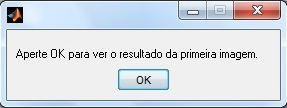
\includegraphics[scale=1.20]{janela1}
		\vspace{2\baselineskip}\vspace{-\parskip}
	
	\item Imagem final do experimento com v\'arios n\'iveis de brilho:\\
		\vspace{2\baselineskip}\vspace{-\parskip}
		\includegraphics[scale=0.50]{imagem2}
		\vspace{2\baselineskip}\vspace{-\parskip}

	\item Janela que mostra ao usu\'ario quantos n\'iveis ele foi capaz de discernir:\\
		\vspace{2\baselineskip}\vspace{-\parskip}
		
\includegraphics[scale=1.0]{janela2}
		\vspace{2\baselineskip}\vspace{-\parskip}
		
 \end{itemize}

\section{Conclus\~ao} 
\label{sec:meth} 
Foi poss\'ivel observar que o olho humano realmente segue algo parecido com o esperado pelo experimento, j\'a que no exemplo que se seguiu o usu\'ario foi capaz de discernir exatamente 24, ou duas d\'uzias, de n\'iveis de cinza.

\end{document}